\subsection{Mathematical Modelling}
The physical problem of the balancing robot is well described by the widely analyzed inverted pendulum model. This system is typically represented as a rigid rod attached to a joint, mounted on a rigid cart that moves in a single direction.

\begin{figure}[H]
	\centering
	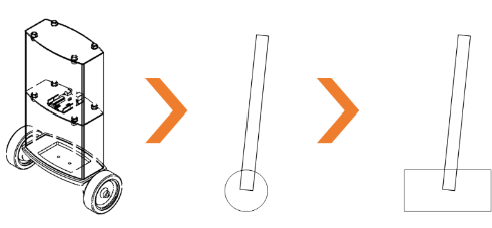
\includegraphics[width=0.6\textwidth]{assets/simplified-inverted-pendulem.png}
	\caption{Simplified inverted pendulum model for the balancing robot \cite{10193276}.}
	\label{fig:pendulum_model}
\end{figure}


For simplification, the wheelbase of the robot is assumed to behave like a cart sliding on a frictionless surface. This modeling approach follows Prasad and Tyagi \cite{prasad_optimal_2014}, and the MathWorks tutorial on the inverted pendulum \cite{matlab_inverted_pendulum}. 

To ease mathematical formulation, the pendulum’s motion is restricted to one degree of freedom, with the angle $\theta$ evolving in the xy-plane, see Figure~\ref{fig:pendulum_model}.

\begin{figure}[H]
	\centering
	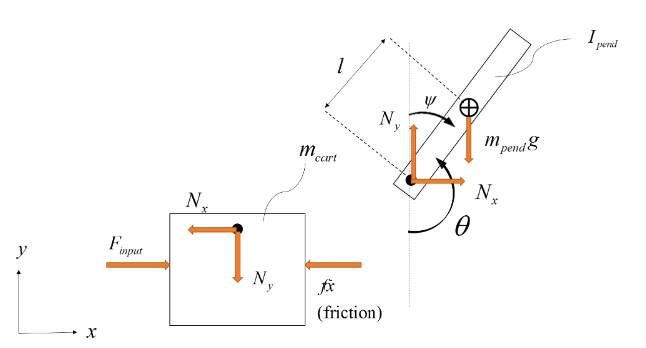
\includegraphics[width=0.6\textwidth]{assets/FBD-inverted-pendulum.png}
	\caption{Free-body diagram for inverted pendulum\cite{10193276}.}
	\label{fig:FBD-inverted-pendulum}
\end{figure}


\subsubsection{State Equations}
The state equations for the system, describing the evolution of the state variables over time, are given by
\begin{equation}
	F_{input} = (m_{cart} + m_{pend}) \ddot{x} + f \dot{x} + m_{pend} l \ddot{\theta} \cos \theta - m_{pend} l \dot{\theta}^2 \sin \theta \label{eq:combined_force}
\end{equation}

\begin{equation}
	(I_{pend} + m_{pend} l^2) \ddot{\theta} + m_{pend} g l \sin \theta = -m_{pend} l \ddot{x} \cos \theta \label{eq:combined_torque}
\end{equation}

\begin{equation}
	\Theta(s) = \underbrace{\frac{\frac{m_{pend} l}{q} s}{s^3 + \frac{f(I_{pend} + m_{pend} l^2)}{q} s^2 - \frac{(m_{cart} + m_{pend}) m_{pend} g l}{q} s - \frac{f m_{pend} g l}{q}}}_{G_\theta(s)} U_{input}(s) \label{eq:transfer_function_psi}
\end{equation}
It is concluded that for all positive value of $l$, $I_{pend}$, $m_{cart}$, $m_{pend}$ and $g$ the system in itself is unstable since it has a pole in the right half plane as can be seen in the pole-zero map in Figure~\ref{fig:pole-zero-map}.

\begin{figure}
	\centering
	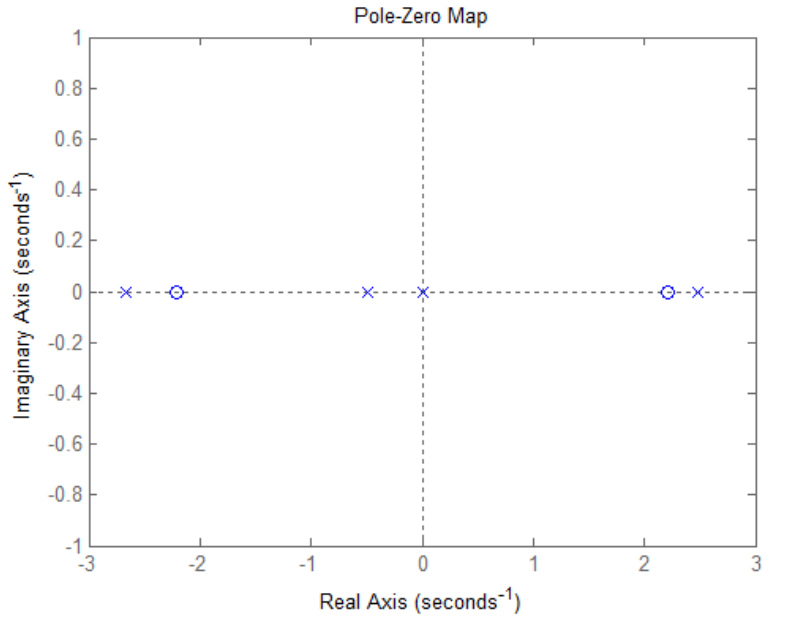
\includegraphics[width=0.7\linewidth]{assets/pole-zero-map}
	\caption{MATLAB-generated pole-zero map of the open loop system $G_{\theta}$ revealing a pole in the right half plane}
	\label{fig:pole-zero-map}
\end{figure}


\subsubsection{Measurement Equation} 
The system's measurement output, which reflects the measured angle, is given by:
\begin{equation}
	{y}(t) = \theta(t) \label{eq:measurement_eq}
\end{equation}
Here, $\mathbf{y}(t)$ denotes the measurement output, which directly corresponds to the system’s angle $\theta(t)$, with no contribution from the gyroscope bias. This measurement model assumes that the system's only observable state is the angle.



\subsubsection{State-space Representation}
The state-space representation of the system is given by:
\begin{equation}
\begin{aligned}
	\underline{\dot{x}}(t) &= \underline{A}.\underline{x}(t) + \underline{B}.\underline{u}(t) \\
	\underline{y}(t) &= \underline{C}.\underline{x}(t) + \underline{D}.\underline{u}(t) \label{eq:state_space_eq}
\end{aligned}
\end{equation}
\begin{itemize}
	\item \textbf{State Vector} $\mathbf{x}(t)$: This vector encapsulates the internal state of the system at time $t$. In this case, it is defined as: 
	\begin{equation}
		\mathbf{x}(t) = \begin{bmatrix} \theta(t) \\ \dot{\theta}(t) \end{bmatrix}
	\end{equation}
	Where $\theta(t)$ represents the measured angle of the system, and $\dot{\theta}_{bias}(t)$ denotes the bias of the gyroscope.
	
	\item \textbf{Input Vector} $\mathbf{u}(t)$: This vector represents the external input given to the system at time $t$. In this case, it is defined as:
	\begin{equation}
		\mathbf{u}(t) = u_{input} 
	\end{equation}
	\item \textbf{State Transition Matrix} $\mathbf{A}$: This matrix describes how the state evolves over time. It is defined as:
\begin{equation}
	\mathbf{A} = \begin{bmatrix}
		0 & 1 \\
		\frac{m_{pend} g l (m_{cart} + m_{pend})}{I_{pend} (m_{cart} + m_{pend}) + m_{cart} m_{pend} l^2} & 0
	\end{bmatrix} \label{eq:state_transition_matrix}
\end{equation}
	The first row indicates that the angle is updated based on its previous value, and the second row shows that the gyroscope bias remains constant in this model.

	\item \textbf{Control Input Matrix} $\mathbf{B}$: This matrix relates the control inputs to the state. In this case, it is defined as:
\begin{equation}
	\mathbf{B} =  \begin{bmatrix}
		0 \\
		\frac{m_{pend} l}{I_{pend} (m_{cart} + m_{pend}) + m_{cart} m_{pend} l^2}
	\end{bmatrix} \label{eq:control_input_matrix}
\end{equation}
	This indicates that there are no direct control inputs affecting the state in this model.
	
	\item \textbf{Measurement Matrix} $\mathbf{C}$: This matrix maps the state vector to the measurement output. It is defined as:
\begin{equation}
	\mathbf{C} = \begin{bmatrix} 1 & 0 \end{bmatrix} \label{eq:measurement_matrix}
\end{equation}
	This means that the measurement output directly reflects the angle, with no contribution from the gyroscope bias.
	
	\item \textbf{Feed-forward Matrix} $\mathbf{D}$: This matrix relates the control input directly to the measurement output. In this case, it is defined as:
\begin{equation}
	\mathbf{D} = 0 \label{eq:feedforward_matrix}
\end{equation}
	This indicates that there is no direct influence of the control input on the measurement output.	

	\item \textbf{Controllability and Observability}: The system is controllable observable if the matrices $S$ and $O$ have full rank.
\begin{equation}
	\mathbf{S} =  \begin{bmatrix} B & AB \end{bmatrix} \label{eq:eq}
\end{equation}

\begin{equation}
	\mathbf{O} =  \begin{bmatrix} C \\ CA \end{bmatrix} \label{eq:eq}
\end{equation}

The rank of $S$ and $O$ confirms that \textbf{the system is controllable and observable} for any positive value of $l$, $I_{pend}$, $m_{cart}$, $m_{pend}$ and $g$.
\end{itemize}
